\documentclass[a4paper,11pt]{report}


\usepackage[T1]{fontenc} % codifica dei font
\usepackage[utf8]{inputenc} % lettere accentate da tastiera
\usepackage[english]{babel} % lingua del documento
\usepackage{lipsum} % genera testo fittizio
\usepackage{indentfirst} % per avere il rientro sulla prima riga del primo paragrafo di una sezione
\usepackage{amsmath} % matematica
\usepackage{amssymb} % matematica
\usepackage{amsthm} % enunciati
\usepackage{booktabs} % tabelle
\usepackage{caption} % tabelle
\usepackage{tabularx} % tabelle
\usepackage{graphicx} % figure
\usepackage{xcolor} % evidenziazione
\usepackage{minted} % codici linguaggi di programmazione
\usepackage{hyperref} % rende cliccabile tutti i riferimenti e permette di scrivere indirizzi internet (sempre ultimo pacchetto)

\linespread{1.5} % spaziamento tra le linee (default 1.0)

\theoremstyle{definition}
\newtheorem{definizione}{Definizione}
\theoremstyle{plain}
\newtheorem{teorema}{Teorema}

\author{Enrico Catalfamo \and Vincenzo Aricò}
\title{Automated AI-based pick-and-place system}

\pagestyle{headings} % plain predefinito su report
\captionsetup{format=hang,labelfont=bf} % bf sulle didascalie sotto figure e tabelle
\setcounter{secnumdepth}{3} % anche le subsubsection saranno numerate e presenti su indice

\begin{document}

\maketitle

\tableofcontents

\chapter{Introduction}
    \section{Premises and goals}
        The project aims, as the title suggests, to create an automated pick-and-place system through the use of Machine Learning techniques. The basic elements involved in the implementation of the project are the following:
        \begin{itemize}
            \item \textbf{A robotic arm}, which is the main player in pick-and-place operations;
            \item \textbf{A conveyor belt}, which conveys the objects to the pre-established point where they are picked up by the robotic arm;
            \item \textbf{A PLC (Programmable Logic Controller)}, responsible for direct control of the robotic arm;
            \item \textbf{A server machine}, which interfaces with the PLC via an Ethernet port to control the robotic arm and on which runs the machine learning model (a convolutional neural network) responsible for object recognition;
            \item \textbf{A client machine}, which connects to the server machine to start or stop the system using a software with a graphical interface, which also allows you to visually monitor the working environment of the robotic arm.
        \end{itemize}
        A more accurate description of the hardware involved (as well as a more exhaustive list) will be made in the subsequent chapters. The basic idea is to have a "proxy" (what we have defined as "server machine"), on which all those operations that generate a certain workload are carried out (management of the webcam flows necessary for monitoring and prediction on objects, loading and starting the machine learning model, management of the robotic arm via commands sent on a socket to the PLC), to which a client can connect, to manage and monitor the system, via an ad-hoc software.
        
        
    \section{High level system architecture}
        The diagram representing the architecture of the system at a high level of abstraction is the following:

        \begin{figure}[H] % H per fissare la figura esattamente in questa posizione
        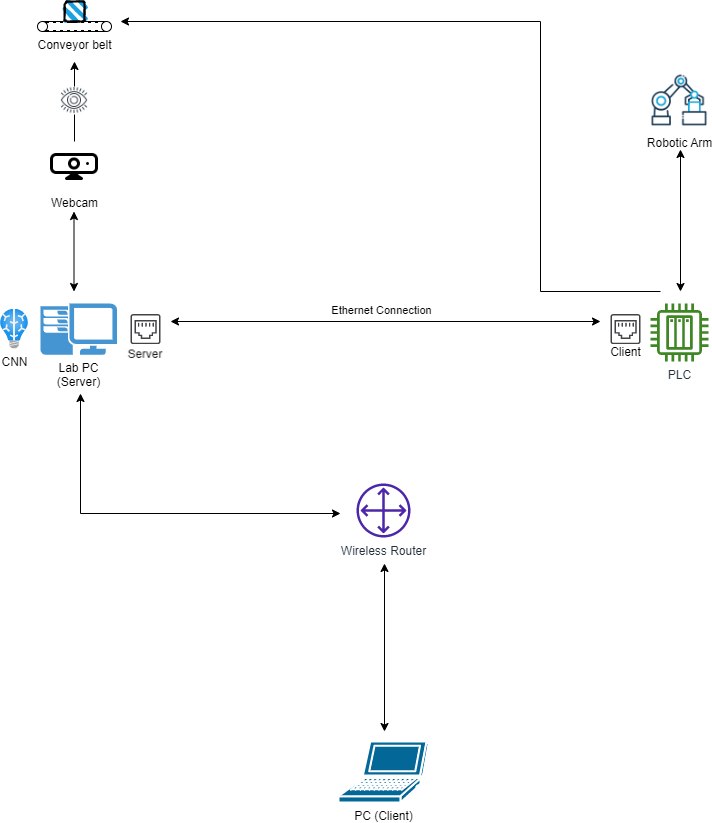
\includegraphics[scale=0.5]{images/architecture.png}
        \centering
        \caption{High level system architecture}
        \end{figure}

        Clearly, the conveyor belt is managed by the PLC through the use of a photoelectric sensor which allows determining the presence or absence of an object to be picked: when an object is detected, the PLC ceases to power the conveyor belt, which stops, allowing the robotic arm to carry out all the necessary operations. More specifically, the logical workflow is the following:
        \begin{enumerate}
            \item The server is started and connects to the PLC on two different sockets: the first one is useful for sending commands to the PLC for managing the robotic arm, while the second one is used by the PLC to send a packet to the server whenever an object is detected, in order to start the server-side AI classification algorithm. In the meantime, the server remains listening on two other sockets (one for exchanging messages aimed at communication, the other for sending the monitoring webcam stream), waiting for a client;
            \item The client connects to the server via the client software GUI, receiving the monitoring webcam stream. By clicking on the start button, the client software sends a \textbf{start} message to the server, which starts the system;
            \item The server waits for an interrupt from the PLC. When it arrives, signaling the presence of an object, a prediction webcam is used to obtain a frame of the object on which to make a prediction using the AI model;
            \item Depending on the prediction, the robot is commanded to pick up and place the object in one position rather than another;
            \item Once the robot has finished this pick-and-place cycle, it starts again from point 3, and continues like this until the client disconnects or decides to stop the system.
        \end{enumerate}

    While the client could be located anywhere, the server machine must be located in a place near the robotic arm as the connection between the PLC and the server machine is made through an ethernet cable.


\chapter{Technologies Involved}
    In this chapter, all the technologies involved in the project will be covered, both hardware and software. We will first list and describe the hardware components used; subsequently, we will review all the software, programming languages and libraries that have come to our aid. It is important to underline that the following is not just a mere list: together with the theoretical notions inherent to the various technologies, certain project choices will be explained and motivated.
    \section{Hardware}
        Although the heart of the project is the software part, it is of great importance to describe all those hardware components that were used and without which it would not have been possible to implement it. In the following section, you will find an explanatory list of these components, together, where necessary, with the reasons behind their choice.
        \subsection{PLC SIMATIC S7-1200}
            The PLC SIMATIC S7-1200 with CPU 1215C AC/DC/RLY (Figure~\ref{plc}) is a PLC produced by Siemens. It is used in the project to realize the sequence control of the robotic arm.
            It is characterized by:
            \begin{itemize}
                \item 14 24V digital inputs;
                \item 10 relay outputs;
                \item 2 analog inputs and 2 analog outputs.
            \end{itemize}
            \begin{figure}[H] % H per fissare la figura esattamente in questa posizione
                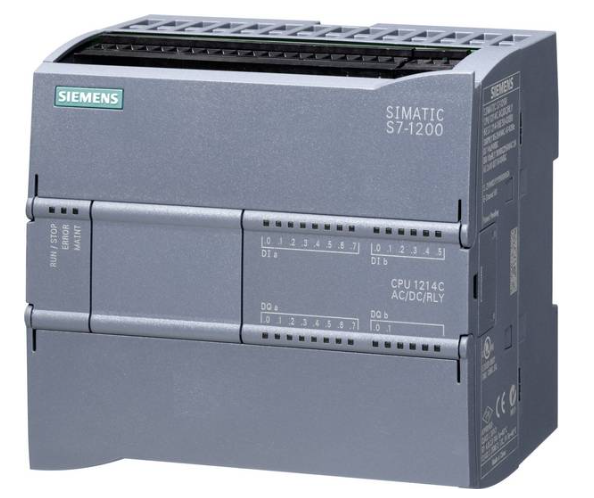
\includegraphics[scale=0.38]{images/plc.png}
                \centering
                \caption{Siemens SIMATIC S7-1200 1215C AC/DC/RLY PLC}
                \label{plc}
            \end{figure}
        \subsection{Fischertechnik 3D-Robot 24V}
            The 3D-Robot 24V (Figure~\ref{robot}) is a robotic arm produced by Fischertechnik. It is a 3-DOF (3 degrees of freedom) robot and in particular it is composed by:
            \begin{itemize}
                \item 1 revolute joint;
                \item 2 prismatic joints (up/down and forward/backward);
                \item 1 gripper as end-effector.
            \end{itemize}
            The robot is characterized by a cylindrical geometry, thus is workspace is a portion of a hollow cylinder.
            \begin{figure}[H] % H per fissare la figura esattamente in questa posizione
                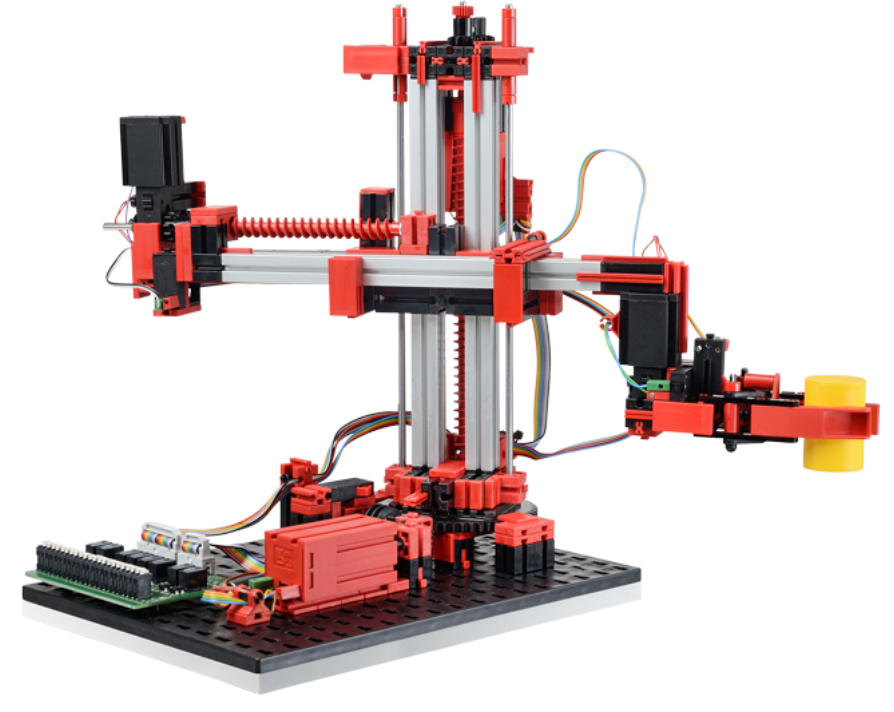
\includegraphics[scale=0.38]{images/robot.png}
                \centering
                \caption{Fischertechnik 3D-Robot 24V}
                \label{robot}
            \end{figure}

            \bigskip
            The robotic arm as four mini switches (Figure~\ref{switch}) that are pressed respectively in four different conditions:
            \begin{itemize}
                \item the gripper is fully open;
                \item the end-effector is completely brought back;
                \item the horizontal arm is completely brought up;
                \item the robot is completely rotated clockwise.
            \end{itemize}
            \begin{figure}[H] % H per fissare la figura esattamente in questa posizione
                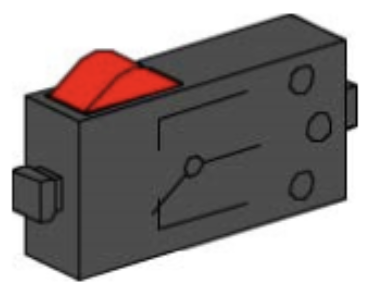
\includegraphics[scale=0.38]{images/switch.png}
                \centering
                \caption{Mini switch}
                \label{switch}
            \end{figure}

            \bigskip
            The robot has two pulse counters, that can be used to understand respectively:
            \begin{itemize} 
                \item how much the gripper is open;
                \item how much the horizontal arm is moved frontward.
            \end{itemize}
            In fact, the pulse counters are switches that are automatically pressed each time a gear involved in the corresponding movement rotate of a certain angle, producing a certain quantity of movement.

            \bigskip
            The robot has two motor encoders (Figure~\ref{encod}) with a maximum frequency of 1 KHz, that can be used to understand respectively:
            \begin{itemize}
                \item how much end horizontal arm is moved down;
                \item how much the robot is rotated.
            \end{itemize}
            \begin{figure}[H] % H per fissare la figura esattamente in questa posizione
                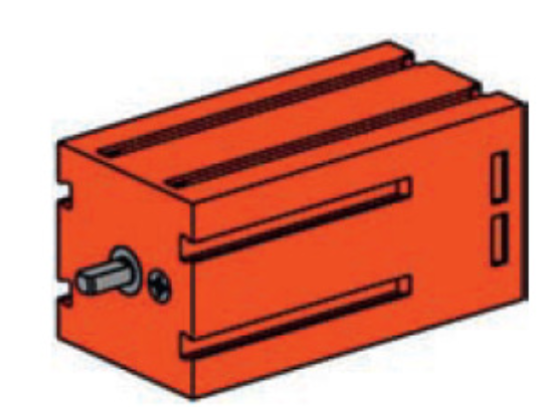
\includegraphics[scale=0.38]{images/encod.png}
                \centering
                \caption{Motor encoder}
                \label{encod}
            \end{figure}
        \subsection{Conveyor Belt}
            The conveyor belt was originally part of an old project and was retrieved at the university, then repurposed for our aims. Almost all the parts that generated unnecessary bulk were removed from the wooden support, as well as all the electronic components that could not have a role in our project. What is left is visible in figure~\ref{nastro}:
            \begin{figure}[H] % H per fissare la figura esattamente in questa posizione
                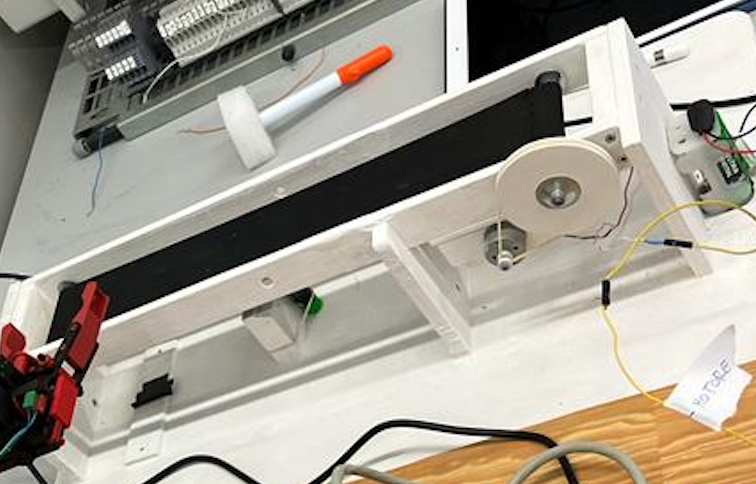
\includegraphics[scale=0.5]{images/nastro.png}
                \centering
                \caption{Conveyor Belt}
                \label{nastro}
            \end{figure}
            To make it usable, it was subsequently necessary to re-tension the belt and replace the "transmission" (a common elastic band). Once done, we took care of checking the voltage necessary to power the DC motor and allow the belt to move at an acceptable speed. After some tests, we came to the conclusion that the optimal voltage for the motor at our disposal was 3V.
        \subsection{Photoelectric sensor E3F-DS10C4}
            \begin{figure}[htbp]
                \centering
                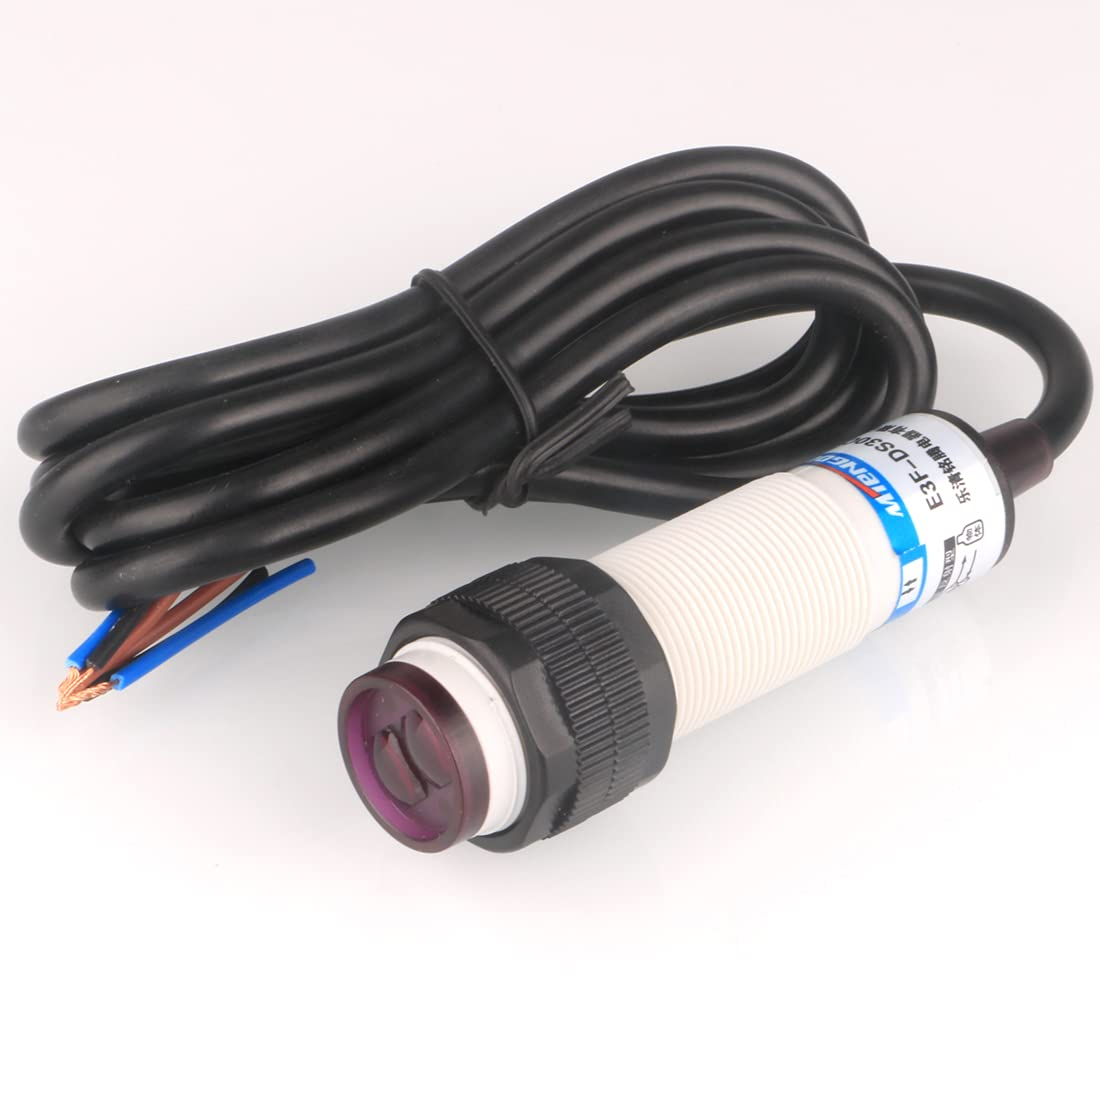
\includegraphics[scale=0.1]{images/sensor.jpg}
                \caption{E3F-DS10C4 sensor}
                \label{sensor}
            \end{figure}
        
            The E3F-DS10C4 sensor (Figure~\ref{sensor}) is a cylindrical diffuse reflection photoelectric sensor with integrated circuit technology, which works as a normally closed switch (normally outputs a high value and switches to a low value when in which it detects the presence of an object). The choice fell on this sensor for the following reasons:
            \begin{itemize}
                \item \textbf{Operating technology}: diffuse reflection. Unlike some inductive and capacitive proximity sensors, photoelectric sensors can detect the presence of objects made of any material (as long as they reflect light), and are therefore more versatile;
                \item \textbf{Supply voltage}: this sensor can be powered with a variable voltage between 10VDC and 30VDC, perfectly in line with the PLC power output (24VDC);
                \item \textbf{Low cost}: the purchase price is relatively low (about 10 euros), especially if you take into account the elasticity, detection speed and robustness of the sensor;
                \item \textbf{Performance}: the sensor is capable of detecting an object placed at 10 cm (adjustable) away by switching in very short times (2.5 ms max);
                \item \textbf{Mounting support}: The geometry of the sensor, together with the included fixing washers, allows the sensor to be mounted and fixed in an optimal way, guaranteeing precision in detections.
            \end{itemize}
            Both the output and the power cable of the sensor were connected to the PLC. Through the ladder diagram, the PLC monitors the status of the relevant input (sensor output) and subsequently carries out all the necessary operations (stop conveyor belt and send packet to the server machine to perform AI prediction of the type of object).
        \subsection{24V Relay}
            \begin{figure}[htbp]
                \centering
                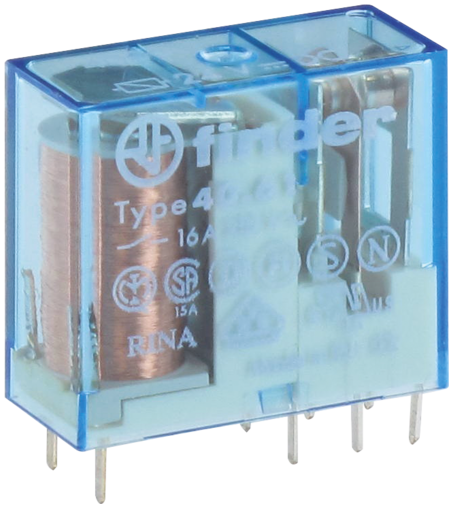
\includegraphics[scale=1]{images/rele.png}
                \caption{The 24V relay used for the project}
                \label{relay}
            \end{figure}
            A 24VDC relay (Figure~\ref{relay}) is an electromechanical device used to control low voltage electrical circuits, operating as a voltage-controlled switch. The operation is very simple: through a 24VDC supply voltage, a solenoid coil is activated, which generates a magnetic field. The interaction between the magnetic field generated by the coil and a mechanical moving contact allows a separate electrical circuit to be opened or closed, allowing the passage of current or interrupting it. \newline
            In our case, the relay was indispensable for controlling the conveyor belt via PLC: direct control, in fact, would not have been possible due to the high output voltages of the PLC; in this way, however, it is possible to connect the PLC output to the relay coil, switching between the 3V and 0V output to power the motor.
            Actually, it would have been possible to connect the sensor output directly to the relay to control the conveyor belt motor. This, however, would have caused the following problems:
            \begin{enumerate}
                \item \textbf{Temporization}: The conveyor belt would restart as soon as the sensor no longer detected the presence of an object. This could have caused collisions between the robot and objects arriving at the picking point and moving on the conveyor belt. By connecting the relay to the PLC output, however, it is possible to insert a timer in the ladder diagram to delay the restart of the conveyor belt.
                \item \textbf{Use of resources}: The server machine would have had no way of being informed about the presence or absence of an object. Consequently, it would have been necessary to take frames from the webcam at a programmed interval to verify the presence of an object and carry out the recognition via AI, using the CPU unnecessarily. 
            \end{enumerate}
        \subsection{USB Webcams}
        As we anticipated in the introduction chapter, in order to realize the project it was necessary to use two webcams: one that took care of environmental monitoring and the other, fixed on the conveyor belt, for object recognition. Since there are no particular requirements for choosing a webcam, except a decent resolution (which is now a common feature of all the devices of this kind on the market), we will not delve into the matter further.
    \section{Software}
        In this chapter we will discuss from a theoretical point of view all the softwares and programming languages used, with the related libraries.
        \subsection{TIA Portal}
            TIA Portal (Totally Integrated Automation Portal) is a software package by Siemens created specifically to develop automation using Siemens products such as PLCs. It is in practice a centralized design environment characterized by a common user interface for all automation tasks with shared services (such as those of configuration, communication and diagnostics) and a single database to which also other software packages, such as SIMATIC WinCC V12, SINAMICS Startdrive V12 and SIMATIC STEP 7 PLCSIM V12, access. The version 15 of the software was used in this project in order to design and upload the control program in the PLC. TIA Portal has a user interface characterized by the presence of two views:
            \begin{itemize}
                \item the portal view;
                \item the project view;
            \end{itemize}

            \begin{figure}[H]
                \centering
            
                \begin{minipage}{0.45\textwidth}
                    \centering
                    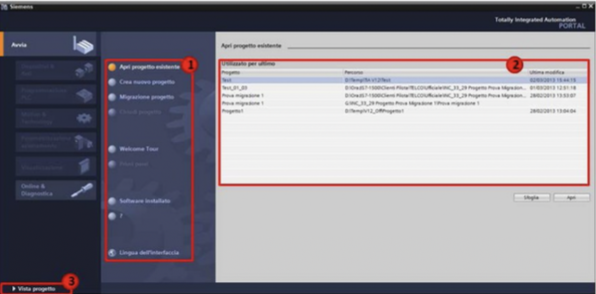
\includegraphics[scale=0.5]{images/portalview.png}
                    \caption*{\textbf{a)} Portal view}
                \end{minipage}
                \hfill
                \begin{minipage}{0.45\textwidth}
                    \centering
                    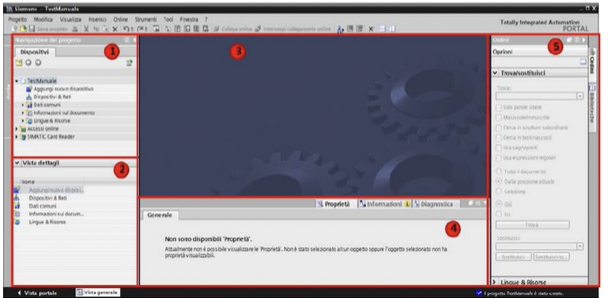
\includegraphics[scale=0.5]{images/projectview.png}
                    \caption*{\textbf{b)} Project view}
                \end{minipage}
            
                \caption{TIA Portal}
            \end{figure}
            
            The portal view is the one that opens automatically when it is launched the TIA Portal and that allows the user to choose which operations he wants to perform with the TIA Portal. It is characterized by the presence of:
            \begin{enumerate} 
                \item a window where it is possible to choose which operation you want to perform;
                \item a selection window related to the selected operation;
                \item a button that allows to switch to the project view.
            \end{enumerate}
            The project view is the working window of the TIA portal that allows the performance of any function within a project; from the project view it is possible to access all the components of the project and quickly navigate within it. It is characterized by the presence of:
            \begin{enumerate}
                \item a window where it is possible to access and navigate all the components of the project;
                \item a window where the content of the component selected in window 1 is visualized;
                \item a window that allows the user to make changes to the project: the editors for writing of the software, the definition of the hardware or the definition of the panel pages based on the context in which the user is located are displayed;
                \item a window where it is possible to view the properties and the details of the objects selected in the window 3;
                \item a window that varies according to the editor that comes presented in window 3 and allows to view and use the TIA Portal Libraries tool.
            \end{enumerate}

        \subsection{Python}
            Python is an object-oriented programming language suitable for application development, scripting, numerical computing and system testing. It is one of the most used languages in the scientific field due to the simplicity of its syntax and the large availability of libraries oriented to experimentation, data analysis and the construction of graphs. In particular, the Numpy and PyPlot libraries are among the most used in this context. Furthermore, with the growing development of artificial intelligence algorithms, many important libraries have also been created such as PyTorch, Keras, Tensorflow and OpenCV, which allow to apply different types of Machine Learning algorithms, not only on numerical or textual data but also on audios, images and videos. \newline
            Python is the language chosen for development of this project because is simple and has very powerful libraries oriented to computer vision, that is the technique able to recognize objects inside images, like the webcam frames.
            \subsubsection{OpenCV}
                OpenCV is an open-source library widely used for image processing and computer vision. It is designed to provide a high-level toolset for developers and researchers to create applications involving real-time image processing. \newline
                Although it is primarily written in C++, it offers interfaces for Python, Java, and MATLAB, providing flexibility and adapting to a wide range of projects. The library contains over 2500 optimized algorithms, covering a wide range of areas such as face detection, object recognition, motion tracking, camera calibration, etc. . \newline
                Its versatility makes OpenCV a popular choice for a wide range of applications. In this context, it was mainly used to interface the server machine with the connected webcams, contributing to the management of the video streaming between the server and the client machine.
            \subsubsection{Zmq}
                ZMQ is a high-speed, low-latency messaging library designed to simplify the development of distributed, scalable applications. It is open-source and offers an asynchronous and stateless communication architecture, which allows the exchange of messages between system components efficiently.\newline
                The library is primarily written in C, but also offers bindings for many other programming languages, including Python. This makes ZMQ accessible to a wide range of developers and allows integration with a variety of technology stacks.\newline
                The ZMQ library provides a variety of communication models, including the publish/subscribe model, abstracting lower-level complexity and providing useful, powerful, and easy-to-integrate functionality within applications. In particular, in the context of this project, ZMQ was used to create a socket with a pub/sub model, useful for managing MJPEG (Motion JPEG) video streaming from the server to the client.
            \subsubsection{Pillow}
                Pillow is an open-source library for image processing in Python. It is a Python Imaging Library (PIL) project fork and offers a wide range of functionalities for image manipulation, editing, and generation.\newline
                Pillow provides a simple and intuitive interface for working with images in different formats, including JPEG, PNG, TIFF, BMP and many others. Images can be opened, saved and converted between different formats, allowing developers to easily manage images with different format requirements. In the context of this project, it was used for the management of received frames on the client side within the graphical interface, created with Tkinter.
            \subsubsection{Tensorflow}
                TensorFlow is an open-source artificial intelligence library developed by Google. It is designed to facilitate the creation and training of machine learning models, especially neural networks, on a wide range of devices and platforms.\newline
                TensorFlow provides a wide range of tools and features for developing AI models. Its main architecture is based on a data flow called a "computational graph", where nodes represent mathematical operations and links between nodes represent data flowing through the system.\newline
                The library supports CPU and GPU computing, allowing developers to leverage the computing power available across devices. Additionally, TensorFlow offers support for distributed computing, allowing you to distribute computation across multiple machines to tackle larger problems and improve performance.\newline
                TensorFlow offers a wide range of machine learning algorithms and pre-built neural networks, such as convolutional neural networks (CNN) and recurrent neural networks (RNN). These algorithms can be used for a variety of tasks, such as, in this case, image classification. By providing pre-trained neural networks on large datasets, Tensorflow allows you to carry out Transfer Learning on tested and functioning models, achieving very high performance. In our case, Tensorflow was used to carry out Transfer Learning on the VGG16 network, training only the Dense layers we inserted.
            \subsubsection{NumPy}
                NumPy is an open-source library for scientific computing in Python. It is widely used to perform efficient operations on multidimensional arrays and provides a wide range of capabilities for scientific data processing.\newline
                NumPy offers a multidimensional array object called ndarray, which allows you to store and manipulate data efficiently. Ndarrays enable efficient operations on large amounts of data, such as vector calculations, element-wise mathematical operations, and broadcasting.\newline
                The library also offers advanced mathematical functions to perform linear algebra, Fourier transforms, statistics, and random number generation operations. These features allow developers to perform complex calculations and data analysis efficiently and accurately. \newline
                In our case, NumPy was mainly used to convert (manually, as well as with reference to data structures) the Matlab code~\cite{matlab} interfacing the PLC and the robotic arm into Python code, avoiding the use of interface libraries between Matlab and Python, helping to make the application robust and monolithic and improving code consistency. Furthermore, the NumPy library was used, together with the other libraries, to manage the images coming from the webcams.
            \subsubsection{Yaml}
                YAML (YAML Ain't Markup Language) is a human-readable data serialization format that is easily parsable by programming languages. It is often used for configuring applications, exchanging structured data, and representing documents. In our project, it was used to create a configuration file that includes all the variable parameters depending on the specific situation (server and PLC IP addresses, interfacing ports, webcam IDs, etc.), in such a way as to allow you to configure the system quickly and, above all, without having to directly modify the code.
\chapter{Implementation}
    Below, we will cover the implementation part of the project, as well as the ways in which the system was actually created. We will first discuss the details of the hardware implementation (all the various circuit connections between the devices that make up the system), then we will move on to describe the features of the code that allow all the components to carry out their work in an effective and coordinated manner.
    \section{Hardware}
        \subsection{Circuit model}
            \begin{figure}[H]
                \centering
                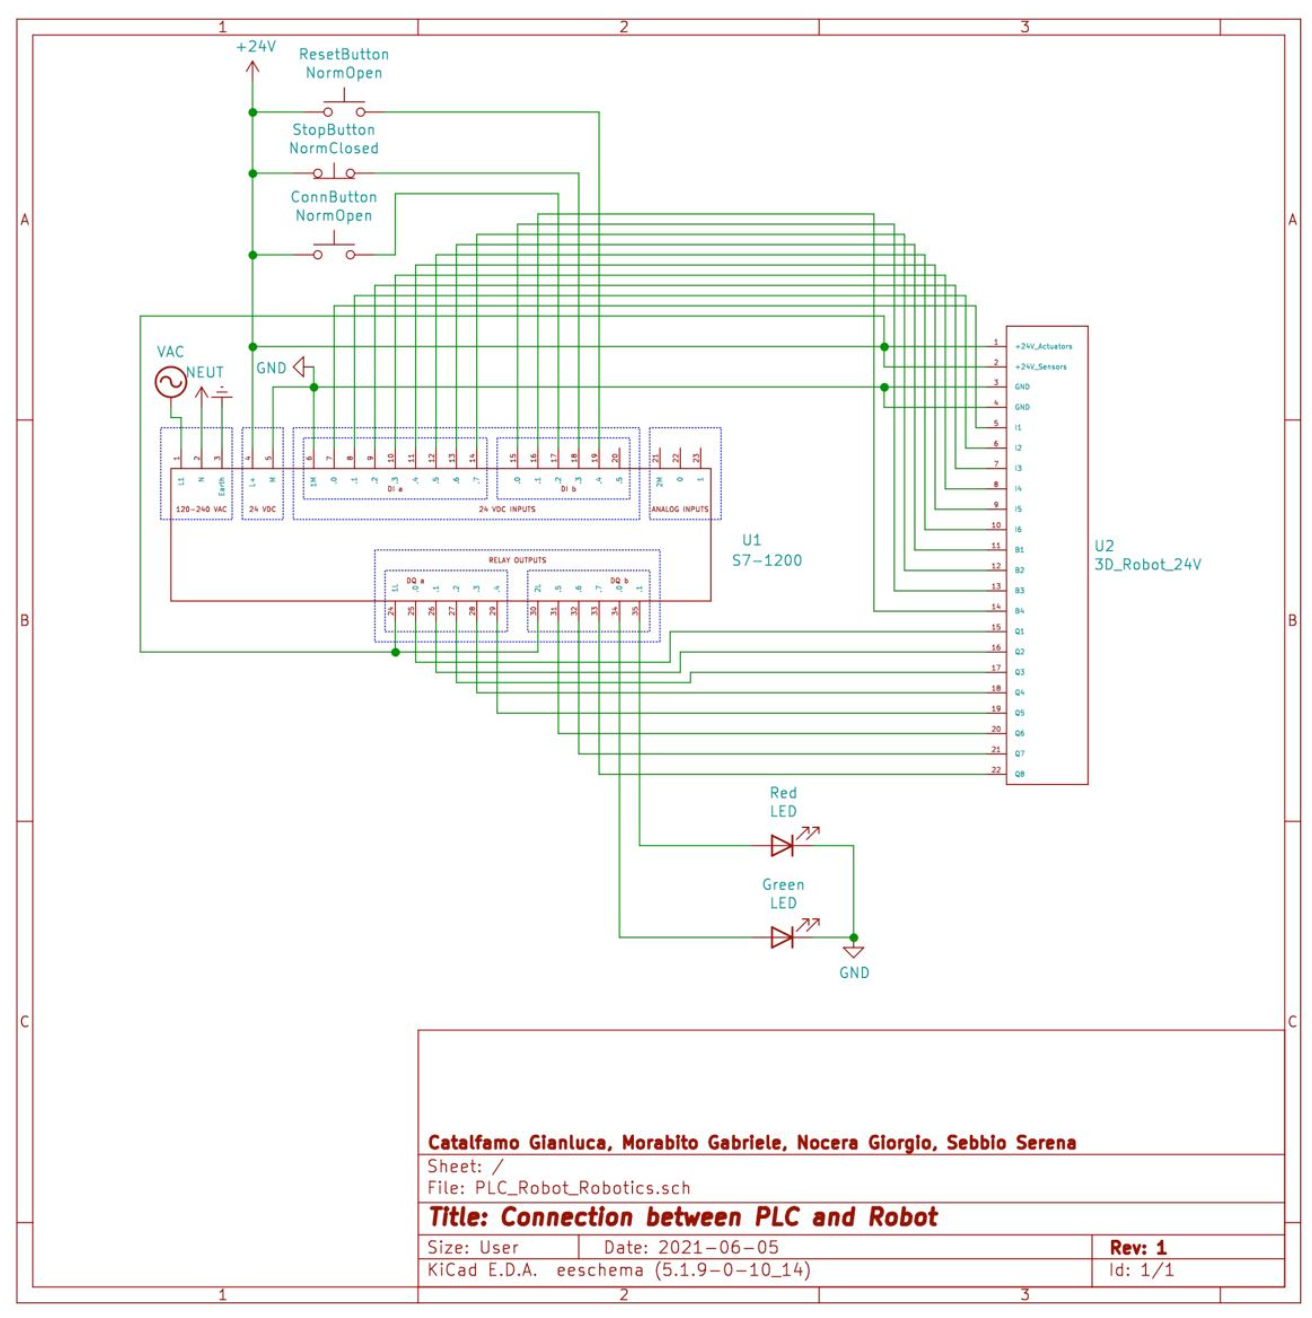
\includegraphics[scale=0.5]{images/schema.png}
                \caption{Initial schematic}
                \label{schema}
            \end{figure} 
            The circuit in Figure~\ref{schema} represents the wiring that was found in the laboratory, physically realized by other students~\cite{schematic}. We started from this circuit to add the hardware related to our system in a "transparent" way (trying not to compromise the circuit already present).
            \subsubsection{Photoelectric sensor E3F-DS10C4 connections}
                The E3F-DS10C4 photoelectric sensor has three wires that need to be connected to the PLC:
                \begin{itemize}
                    \item \textbf{power supply (brown)}: connected to pin L+ (24 VDC port) of the PLC;
                    \item \textbf{ground (blue)}: connected to pin M (24 VDC port) of the PLC;
                    \item \textbf{output signal (black)}: connected to the last available input pin, i.e. pin DIb5 (24 VDC INPUTS port) of the PLC.
                \end{itemize}
                \begin{figure}[H]
                    \centering
                    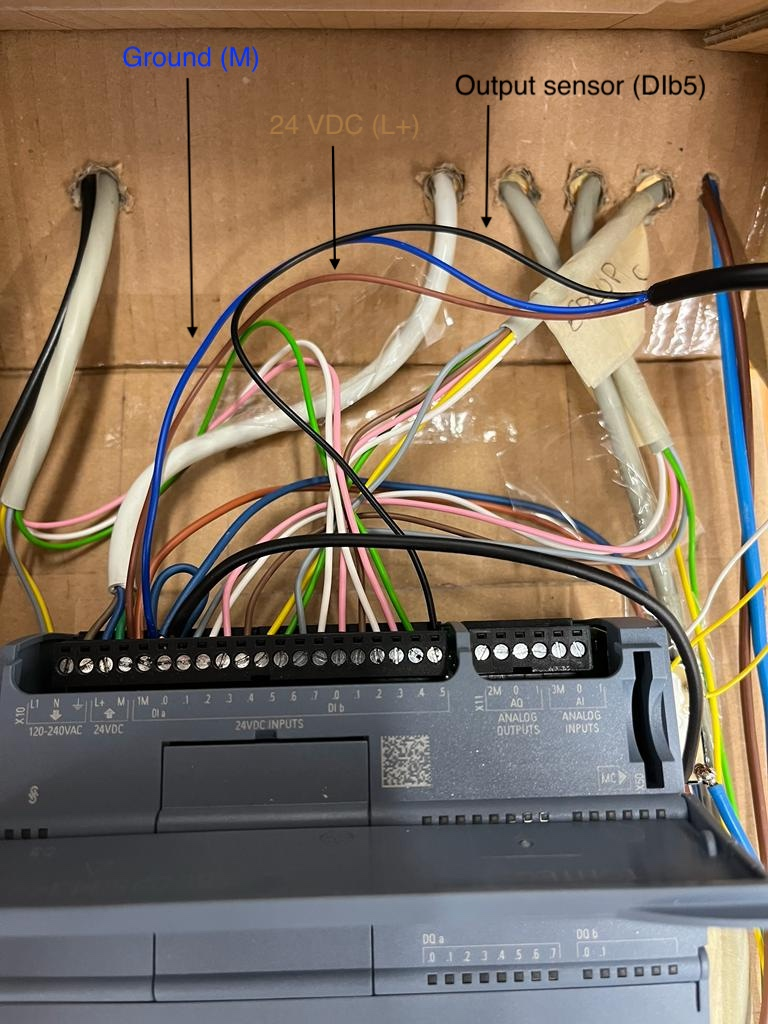
\includegraphics[scale=0.35]{images/sensorconn.jpeg}
                    \caption{E3F-DS10C4 connections}
                \end{figure} 
            \subsubsection{Conveyor Belt connections}
                The DC motor, capable putting in motion the conveyor belt, must be powered with 3 VDC (2 1.5 VDC batteries). The power supply to the motor must be immediately interrupted when an object is detected by the photoelectric sensor, while it must be restored after a few seconds when the detected object is picked up by the manipulator, in order to avoid collisions between the end-effector and the objects arriving at the pick position.
                Power to the motor is provided by a relay controlled by voltage from a 24 VDC output pin of the PLC. Since there were no output pins available, the red LED connected to pin DQb1 (RELAY OUTPUTS port) was disconnected in order to use the pin to control the relay input voltage. This is how it works:
                \begin{itemize}
                    \item \textbf{pin DQb1 = 0 VDC}: object not detected, therefore the conveyor belt can be powered;
                    \item \textbf{pin DQb1 = 24 VDC}: object detected, therefore power to the conveyor belt must be immediately cut off.
                \end{itemize}
                To supply or interrupt power to the conveyor belt, two separate circuits are necessary, as in Figure~\ref{schemarele}. The circuit on the left (with the battery) will power the motor and close ("activate") when \textbf{pin DQb1 = 0 VDC}, while the circuit on the right (without the battery) will cut power to the motor and close ("activate") when \textbf{pin DQb1 = 24 VDC}. Obviously, when one of the two circuits is closed, the other one will be open.
                \begin{figure}[H]
                    \centering
                    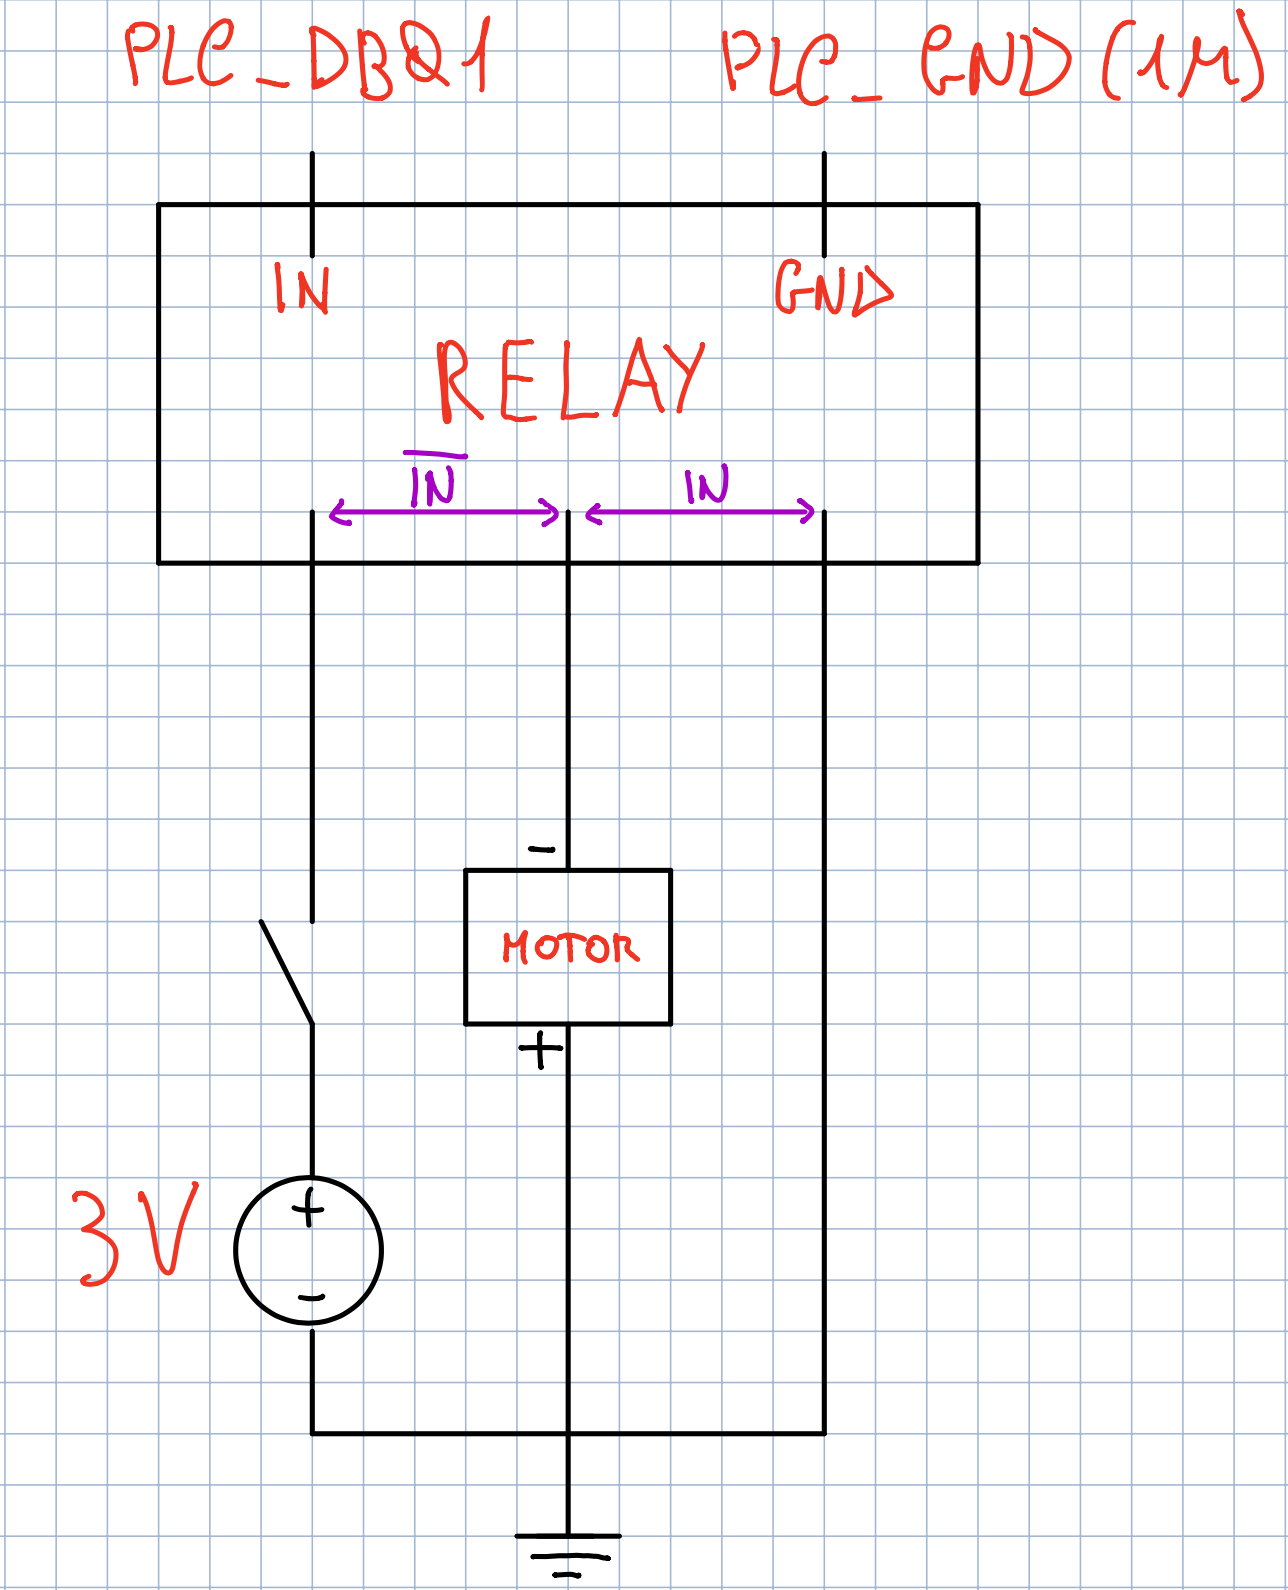
\includegraphics[scale=0.35]{images/schemarele.png}
                    \caption{Relay schematic}
                    \label{schemarele}
                \end{figure} 
                \begin{figure}[H]
                    \centering
                    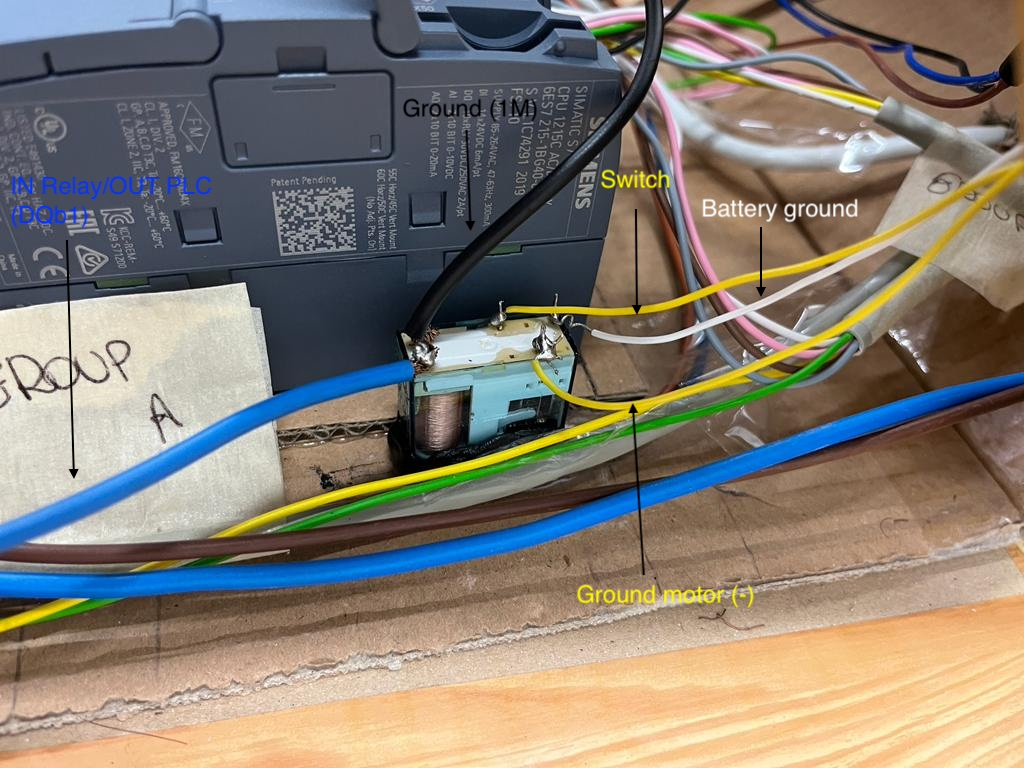
\includegraphics[scale=0.35]{images/releconn.jpeg}
                    \caption{Relay connections}
                \end{figure}
                \begin{figure}[H]
                    \centering
                    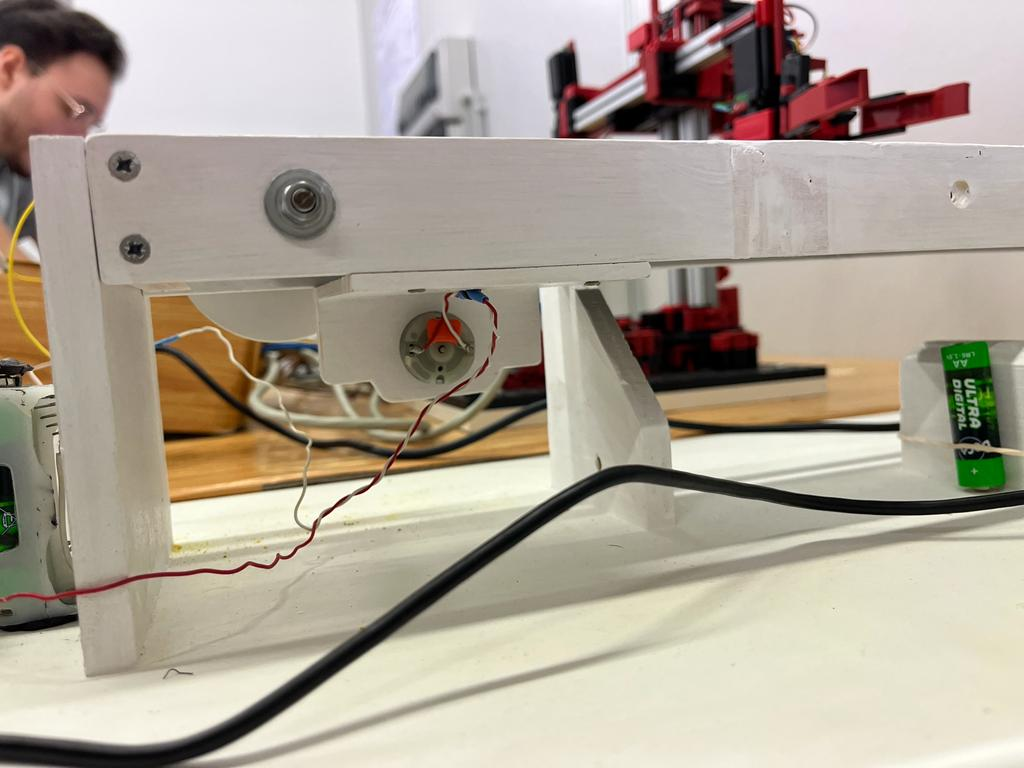
\includegraphics[scale=0.3]{images/motorposition.jpeg}
                    \caption{Motor position on conveyor belt}
                \end{figure}
                \begin{figure}[H]
                    \centering
                    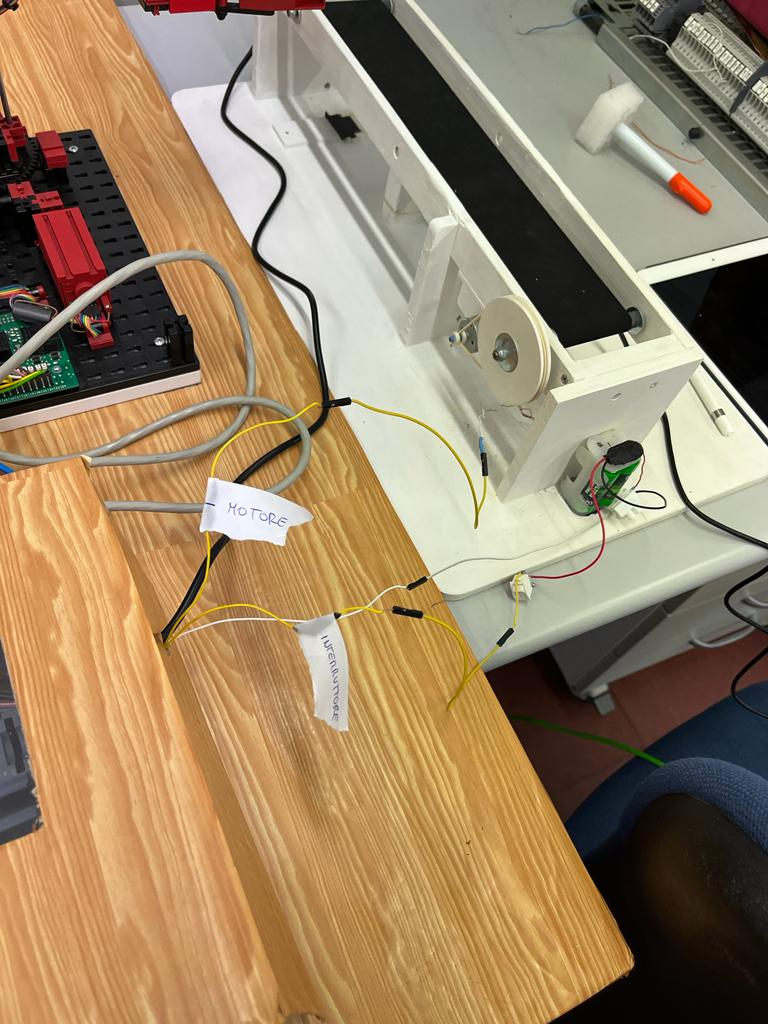
\includegraphics[scale=0.35]{images/namewires.jpeg}
                    \caption{Labeled relay connections to separate circuits}
                \end{figure}
        \subsection{Scene image}
            \begin{figure}[H]
                \centering
                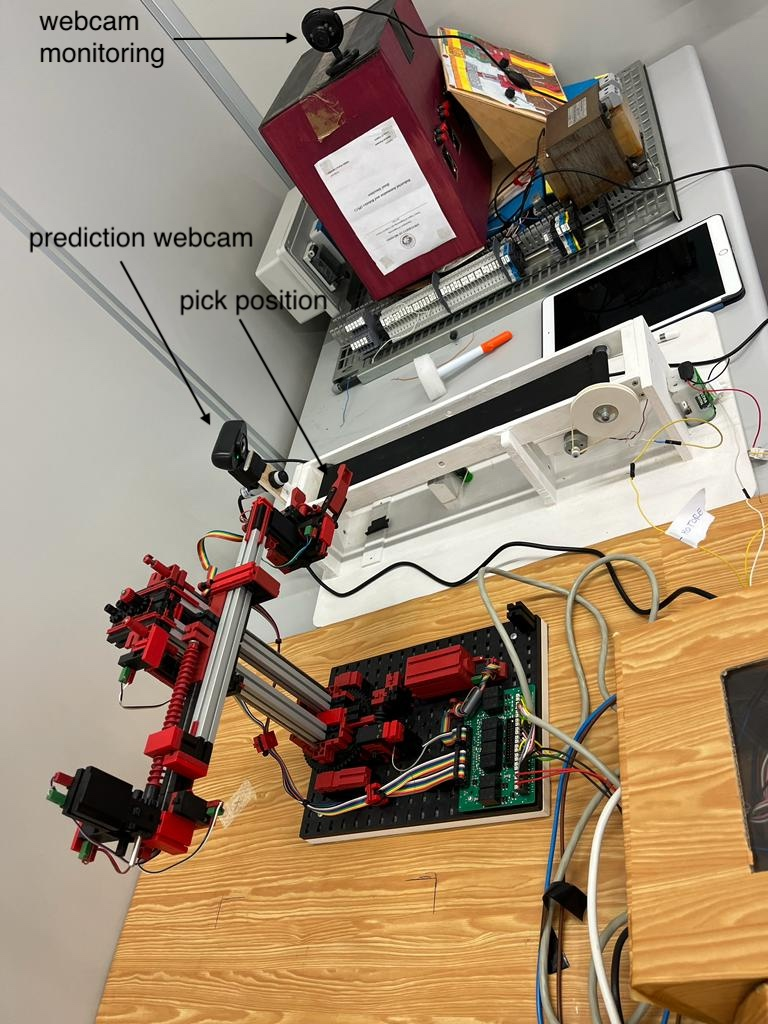
\includegraphics[scale=0.5]{images/scene.jpeg}
                \caption{Scene image}
            \end{figure}
    \section{Software}
        The software is mainly composed by the following elements:
        \begin{itemize}
            \item The Communication module, which defines a JSON-based application-level communication protocol to allow the exchange of system control messages between client and server;
            \item The ServerClass class, which is responsible for orchestrating all the functions related to environment monitoring, robot movement and object recognition;
            \item A convolutional neural network, which is called at the appropriate time to perform object recognition;
            \item A script for the client, which generates a graphical interface through which it is possible to connect to the server, start/stop the system and monitor its behavior;
            \item A configuration file, containing all the parameters relating to the connections between client, server and PLC, which allows the system to be reconfigured easily and quickly depending on the context.
        \end{itemize}
        Server-related tasks are conveniently handled by separate threads, creating a multi-threaded application.
        \subsection{AI Model}
            To simplify and abstract the object recognition part, foam rubber cubes were created on which a geometric shape between a square and a triangle was drawn. Recognizing the object, therefore, boils down to recognizing the geometric shape present on the cube. The point at which the cube is released once grabbed by the robot depends on the latter. \newline
            \begin{figure}[H] % H per fissare la figura esattamente in questa posizione
                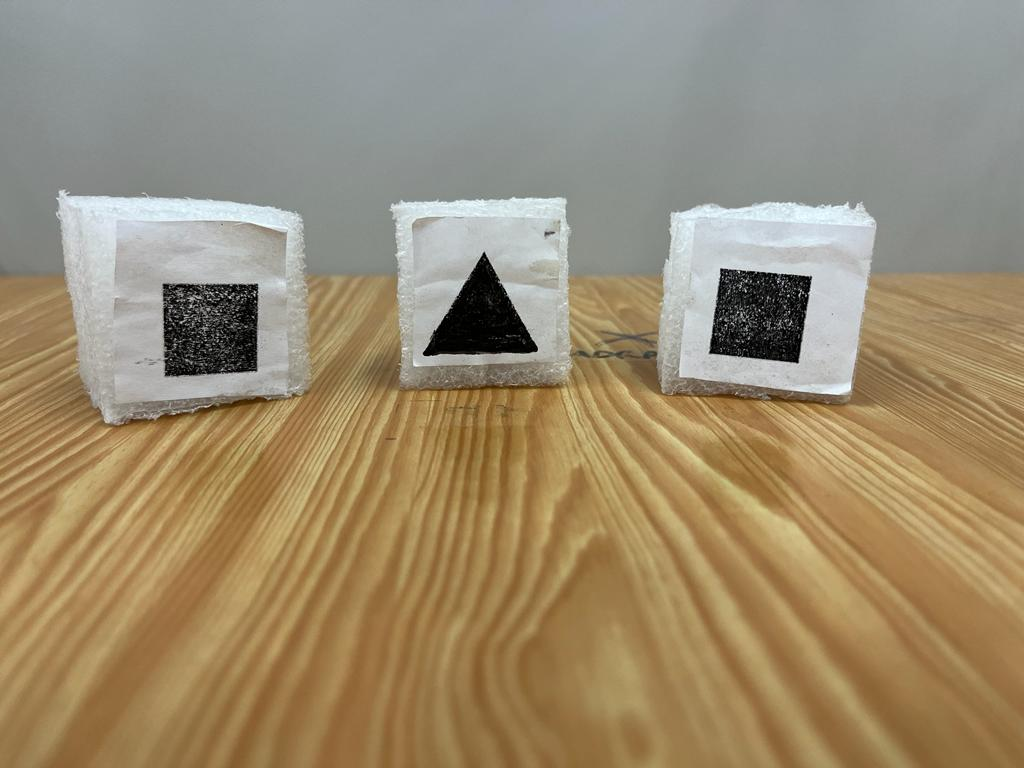
\includegraphics[scale=0.15]{images/cubi.jpeg}
                \centering
                \caption{Cubes}
            \end{figure}
            \begin{figure}[H] % H per fissare la figura esattamente in questa posizione
                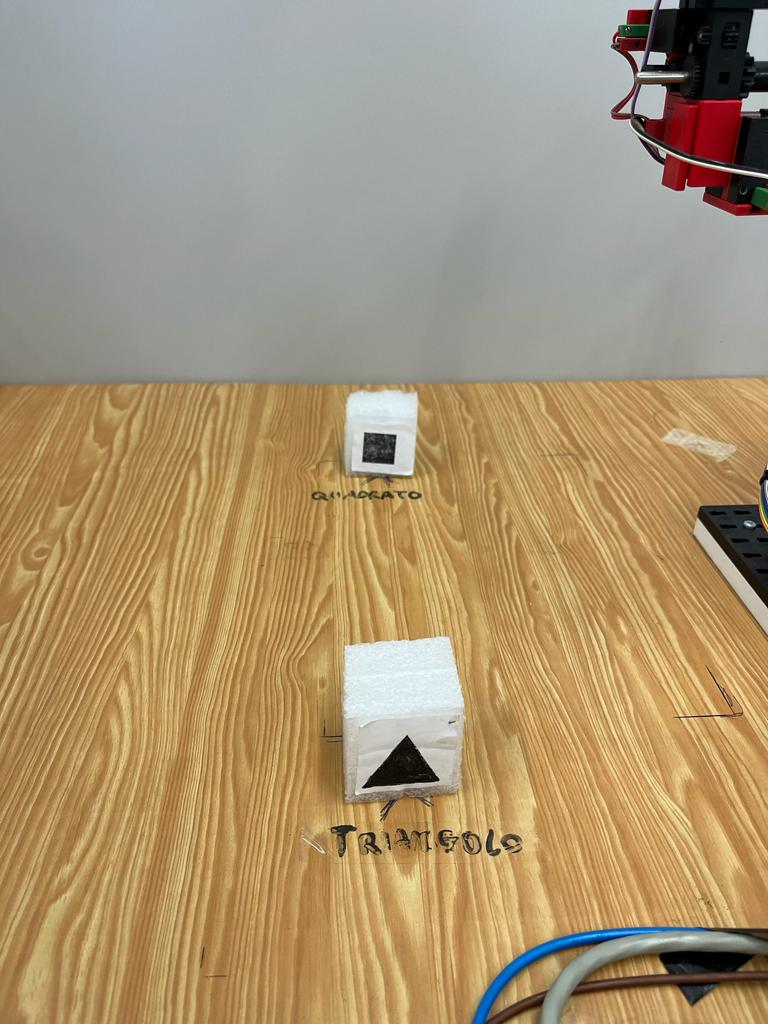
\includegraphics[scale=0.3]{images/targets.jpeg}
                \centering
                \caption{Targets}
            \end{figure}
            The model used for shape recognition is a convolutional neural network, in particular the VGG16 network, which has been modified in its final Dense layers to adapt it to the task of our interest. The network is able to distinguish between the two geometric shapes, as well as verify that a geometric shape is actually present: if this does not happen, the system must notify the event. This implies that the network must be trained in such a way to be able to detect the absence of geometric shapes.
            \subsubsection{Creating the dataset}
                We could have created the dataset "by hand", taking pictures of the previously crafted cubes and feeding them to the network during the learning phase. However, this approach would inevitably have involved the use of a small dataset, leading to overfitting and, therefore, poor performance in the inference phase (the network would not have been able to generalize correctly). The path we preferred to follow, however, is that of using a synthetic dataset. \newline
                This dataset was obtained using an image generator~\cite{githubdata} containing geometric shapes (randomly rotated and scaled) of different colors on a homogeneous background.
                The software, however, creates images containing not only triangles and squares, but also other geometric shapes. Since the generation of images takes a relatively long time, especially when the number of examples to be generated is quite high, it was necessary to make some slight modifications to the code to ensure that only the geometric shapes of interest to us were generated. Furthermore, to make the network able to recognize the absence of geometric shapes, we ensured that images were generated without geometric shapes in the background.
                With these methods, a balanced dataset of 15000 images (5000 per class) was generated.

                \begin{figure}[H]
                    \centering
                
                    \begin{minipage}{0.2\textwidth}
                        \centering
                        
\includegraphics[scale=0.15]{images/data3.jpeg}
                        \caption*{\textbf{a)} Triangle}
                    \end{minipage}
                    \hfill
                    \begin{minipage}{0.2\textwidth}
                        \centering
                        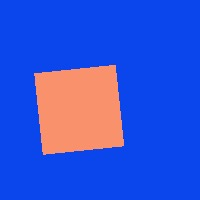
\includegraphics[scale=0.15]{images/data2.jpeg}
                        \caption*{\textbf{b)} Square}
                    \end{minipage}
                    \hfill
                    \begin{minipage}{0.2\textwidth}
                        \centering
                        
\includegraphics[scale=0.15]{images/data1.jpeg}
                        \caption*{\textbf{c)} Absence}
                    \end{minipage}
                
                    \caption{One image per class}
                \end{figure}
            
            \subsubsection{Training the model}
                The model consists of an input layer with shape (200, 200, 3), a rescaling layer to bring the pixels into a range between 0 and 1, the pretrained hidden layers of the VGG16 network and three final dense layers to train (one with 32 neurons, one with 16 and the last one, of course, with 3 neurons and softmax activation function). The Adam optimizer was used, with a starting learning rate of 0.0001. The reference metric is accuracy.
                The network was trained for a single epoch, to avoid overfitting. The ratio between the cardinality of the training dataset and that of the test dataset is 80-20: 12000 samples to train the network and 3000 to test its generalization capabilities. The model achieved an accuracy of 94\% on the training set and 97.5\% on the test set.
        \subsection{The Communication module}
            The Communication module allows client and server to exchange messages about system control in a simple way. Inside, two functions are defined: receive() and send().
            Both functions take advantage of the tools made available by Python sockets and the JSON module. The send() function, very simply, creates a dict using the input parameters, transforms it into JSON, serializes it and sends it to the socket.
            \begin{figure}[H]
            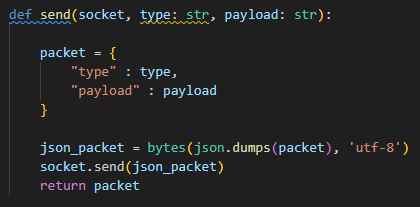
\includegraphics[scale=0.7]{images/send function.png}
            \centering
            \caption{The send() function}
            \end{figure}
            The receive() function listens on the socket (collecting packets) until it has received the entire JSON. This is verified, thanks to the fact that JSON is highly structured, by counting the curly braces contained in the received packets. When the counter reaches zero (i.e. when as many opening braces as closing braces have been received), the JSON is returned in full (as a dict) to the caller.
            \begin{figure}[H]
            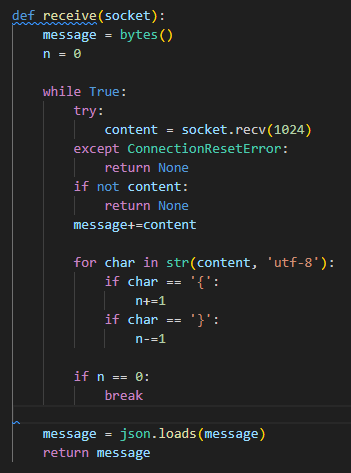
\includegraphics[scale=0.7]{images/receive function.png}
            \centering
            \caption{The receive() function}
            \end{figure}
        \subsection{Client-side code}
            The client-side code is very simple. Through Tkinter, a graphical interface is created, with the aim of giving the user a simple and intuitive means for managing the system. The script takes the server connection parameters from the configuration file and defines some main elements:
            \begin{itemize}
                \item A "Connect" button, which allows you to connect to the server, receiving the video stream and receiving/sending messages related to system control;
                \item A "Disconnect" button, which closes both sockets (both the one related to the video stream and the one related to the exchange of control messages);
                \item A "Start" button, which starts the system (sending a control message to the server), allowing the robot to start sorting the cubes;
                \item A "Stop" button, which stops the system;
                \item A window showing the video stream of the working environment;
                \item A box in which any messages returned by the server are shown.
            \end{itemize}
            \begin{figure}[H]
                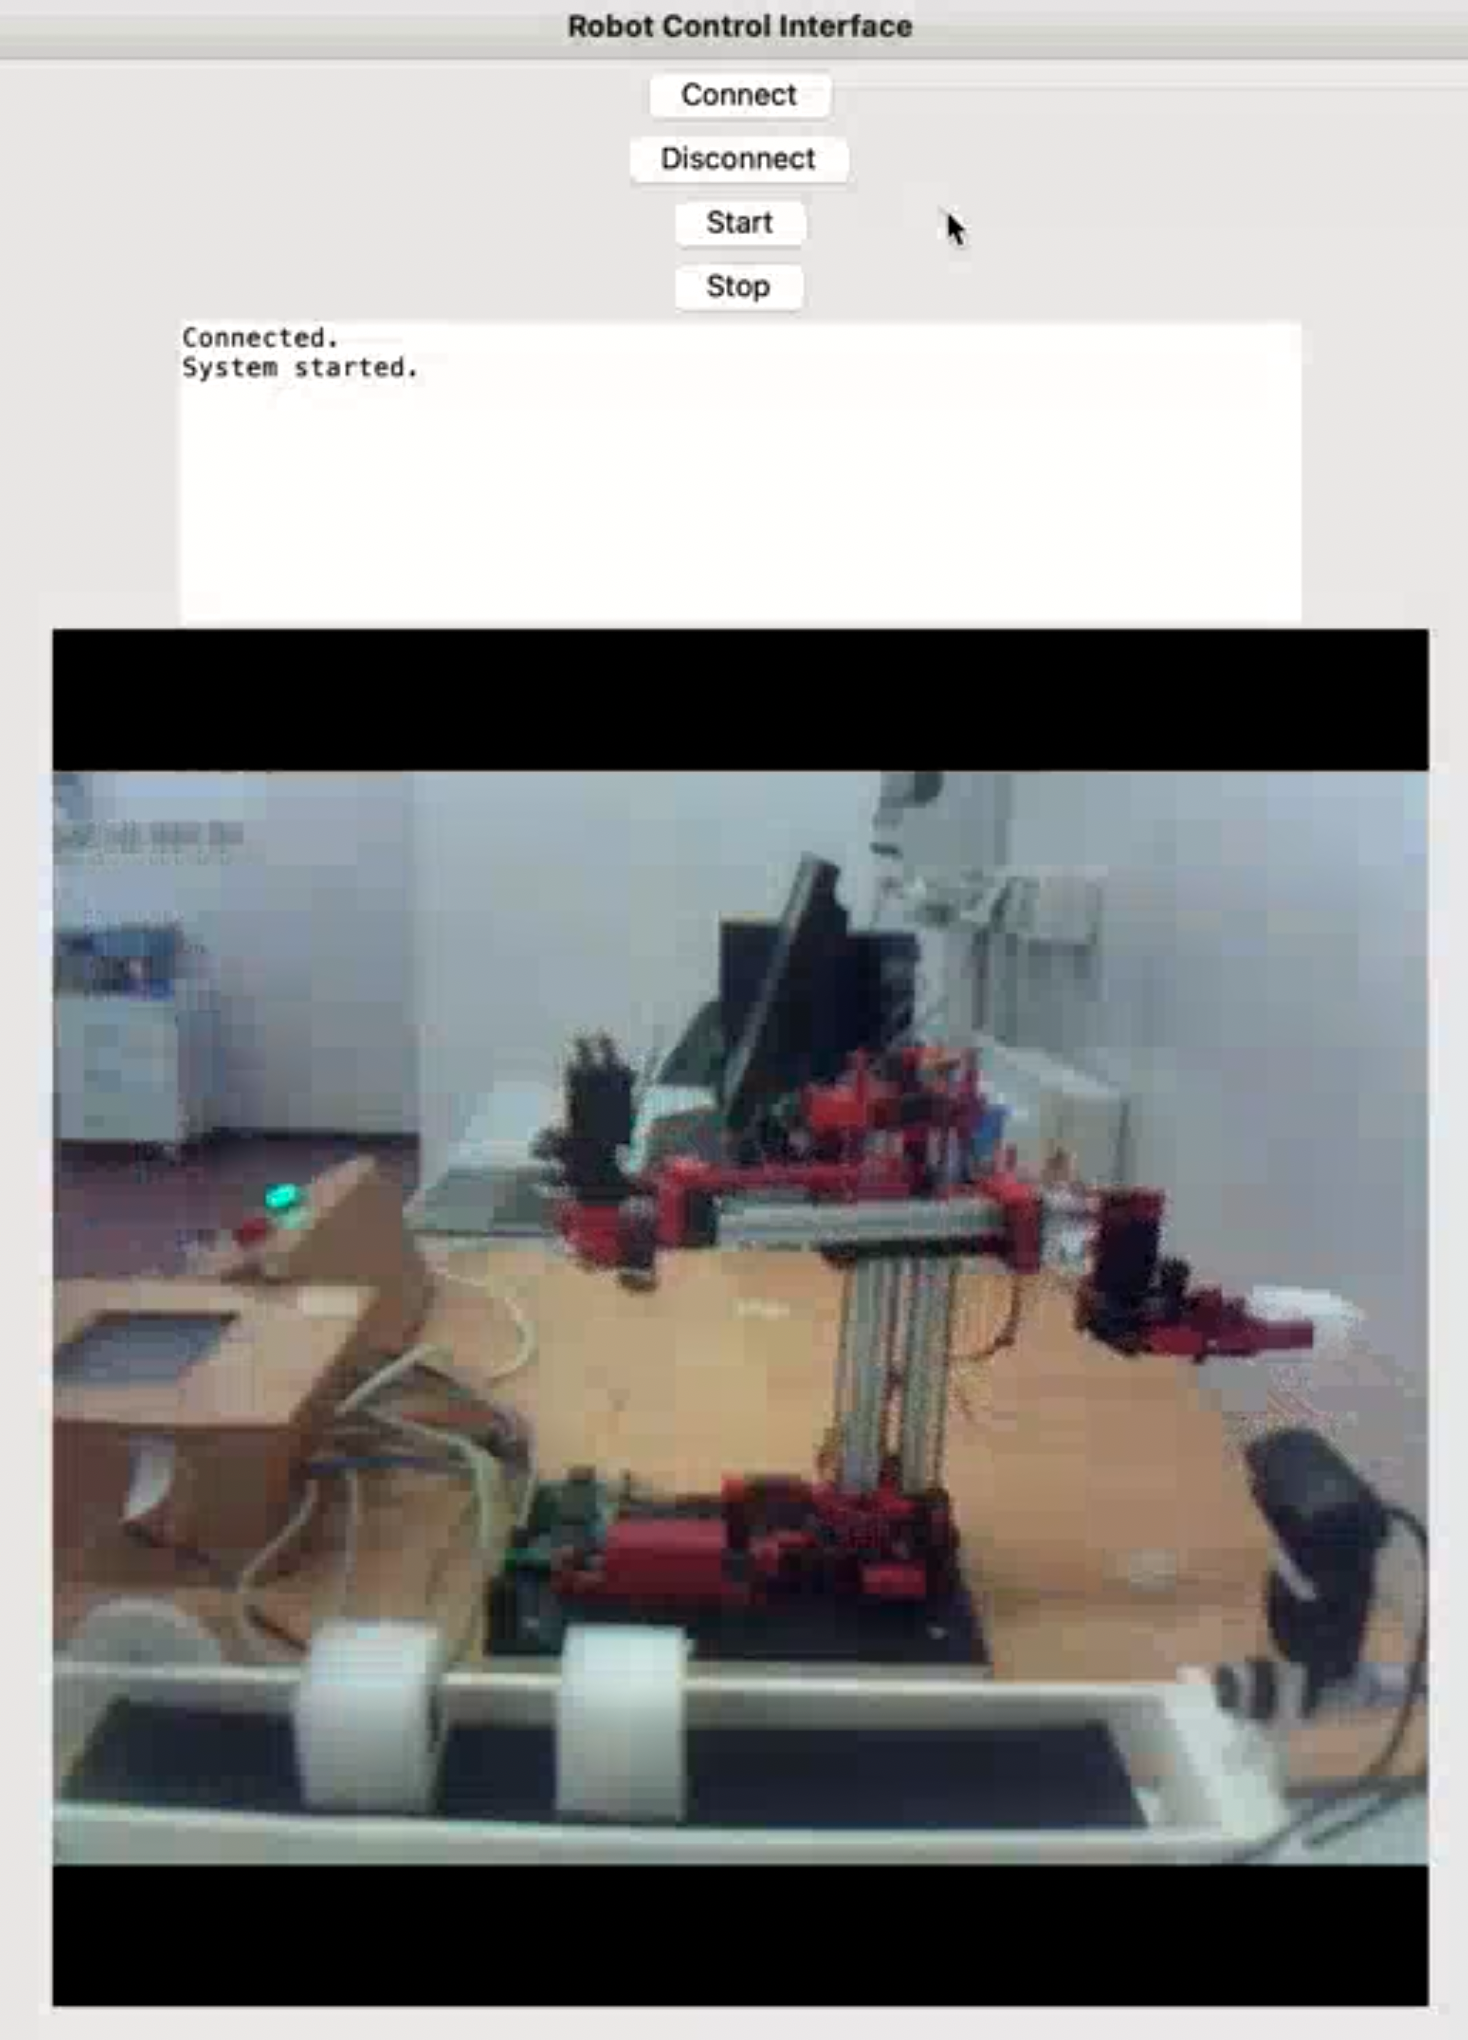
\includegraphics[scale=0.4]{images/interface.png}
                \centering
                \caption{Client control interface (GUI)}
            \end{figure}
            All these elements (in particular the video streaming window and the message box) are updated every 4 milliseconds, following the logic defined in the update\_root() function.
            \begin{figure}[H]
            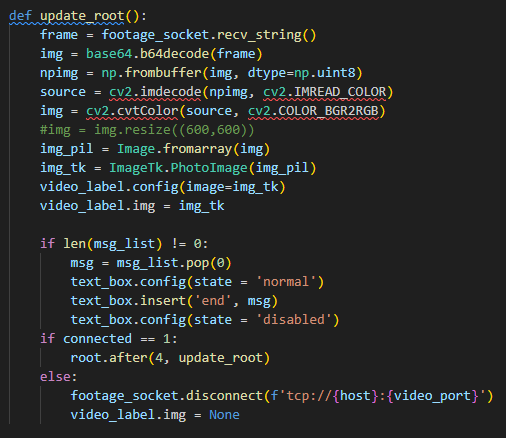
\includegraphics[scale=0.7]{images/update_root.png}
            \centering
            \caption{The update\_root() function}
            \end{figure}
            The function takes a frame from the video stream socket, shows it on the screen (replacing the previous one) and checks that there are elements in the control message queue, in which case it shows them in the related box. The GUI update, which occurs every 4 milliseconds, is carried out only if the client is connected to the server (otherwise, it is not necessary to update the screen).
            The other functions defined in the script, however, simply deal with connecting or disconnecting the client from the server, updating the state variables accordingly, or sending specific control messages to the server via the Communication module (start and stop, specifically).
            
            \begin{figure}[H]
            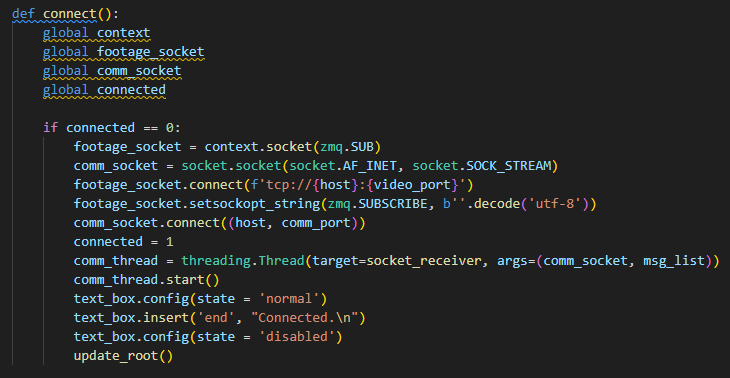
\includegraphics[scale=0.7]{images/connect func.png}
            \centering
            \caption{The connect() function}
            \end{figure}
            
            \begin{figure}[H]
            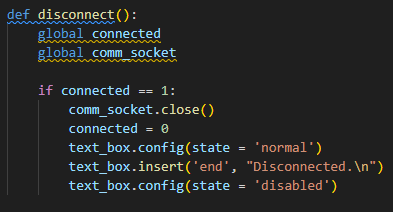
\includegraphics[scale=0.7]{images/disconnect func.png}
            \centering
            \caption{The disconnect() function}
            \end{figure}
            
        \subsection{Server-side code}
        The server-side script imports the ServerClass class, takes the configuration parameters from the configuration file, creates a ServerClass instance and calls the start method to instantiate the server. \newline
        The ServerClass class defines two methods: the initialization method (\_\_init\_\_), and the start method, which instantiates and runs the server.
        The input parameters of the \_\_init\_\_ function must be contained in a dictionary, and are:
        \begin{itemize}
            \item The IP address of the network interface on which the server to which the client must connect will be instantiated, as well as the related ports;
            \item The IP address of the network interface on which the server to which the PLC must connect will be instantiated, as well as the related ports.
        \end{itemize}
        Subsequently, in the same function, all the objects necessary for the correct functioning of the server are created, namely:
        \begin{itemize}
            \item Two cv2.VideoCapture objects, which provide a handle for the two webcams connected to the system (object recognition and monitoring of the working environment);
            \item The sockets to be bound to the IPs and ports above;
            \item A variable containing, as a string, the current state of the system (initially "STOP");
            \item A numpy array containing the initial position of the robotic arm (initialized to zero);
            \item Two Thread objects for separate management of the robot's movement and video streaming;
            \item A threading.Event object to ensure correct synchronization between system operation and commands sent by the client.
        \end{itemize}
        \begin{figure}[H]
        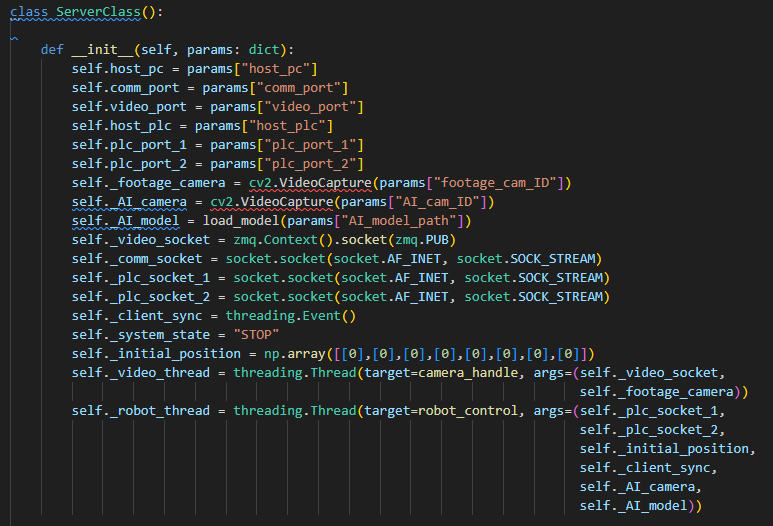
\includegraphics[scale=0.7]{images/Serverclass init.png}
        \centering
        \caption{ServerClass \_\_init\_\_ function}
        \end{figure}
        The start() function binds the server sockets to the addresses and ports defined in the previous function and starts the two threads related to the robot movement and the video stream, then listens on the communication socket with the client, waiting for a connection. Once the client is connected, the server waits to receive messages from it, as a result of which it updates its state and interacts with the robot's movement thread via the threading.Event object, stopping or starting the sorting of the cubes.

        \begin{figure}[H]
        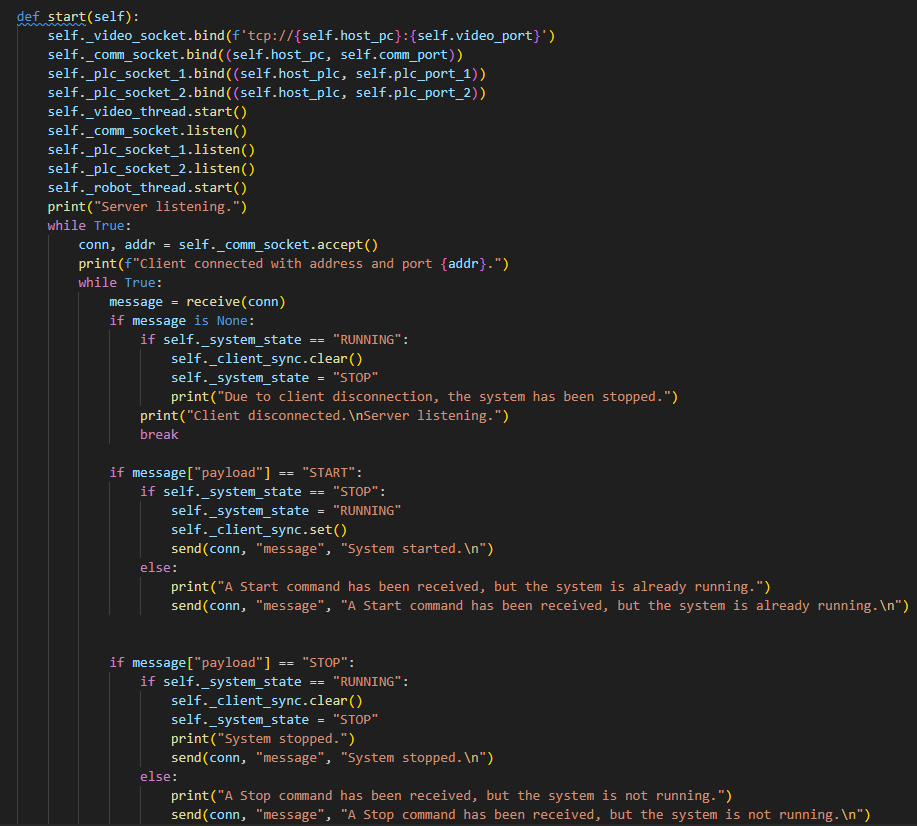
\includegraphics[scale=0.6]{images/Serverclass start.png}
        \centering
        \caption{ServerClass start() function}
        \end{figure}
        The camera\_handle() function, linked to a separate thread, does nothing more than taking a frame from the webcam, encoding it first in JPEG, then in base64 and finally sending it over the socket, ready to be picked up by the client. This is done every 0.05 seconds.
        \begin{figure}[H]
        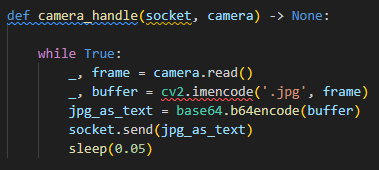
\includegraphics[scale=0.7]{images/camera handle.png}
        \centering
        \caption{The camera\_handle() thread function}
        \end{figure}
        The robot\_control function, tied to the robot control thread, works as follows:
        \begin{itemize}
            \item When the thread is started, it listens on the socket, waiting for the PLC to connect;
            \item Once the PLC is connected, it verifies that the system is in running state, checking that the event object is set;
            \item If the system is running, it waits to receive notification from the PLC about the presence of an object in the pick position;
            \item Once it receives this message, it takes a frame from the object recognition webcam, withdraws the part of the image containing the geometric shape and feeds it to the ML model;
            \item Depending on the prediction, the robot is commanded to follow one path rather than another. If the predicted class is the third, corresponding to the absence of geometric shapes, this is notified to the server application, inviting the operator to remove the object from the conveyor belt.
        \end{itemize}
        The function that actually carries out the movement of the robotic arm, move\_robot, is nothing but the Python version of the Matlab function of the same name defined in the project which can be consulted at the link~\cite{matlab} in the bibliography.
        \begin{figure}[H]
        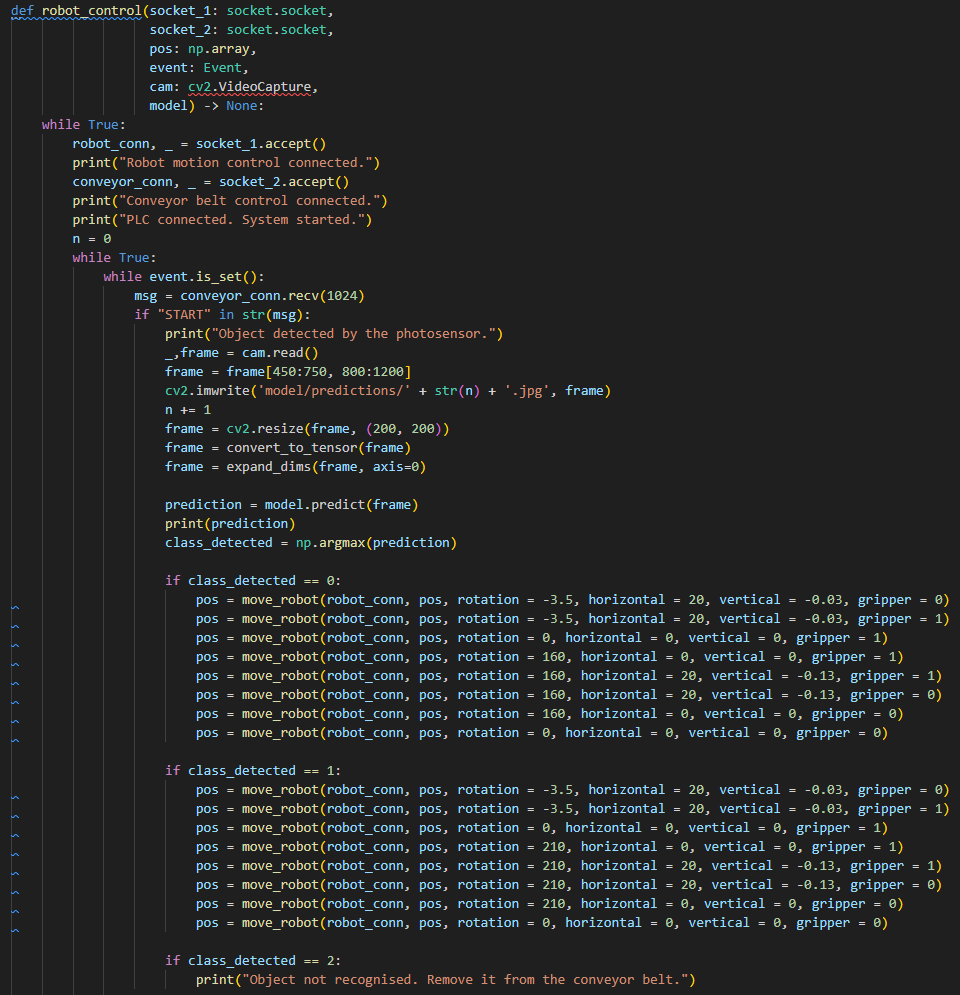
\includegraphics[scale=0.6]{images/robot control.png}
        \centering
        \caption{The robot\_control() thread function}
        \end{figure}
        
        \subsection{Configuration file}
        \begin{figure}[H]
        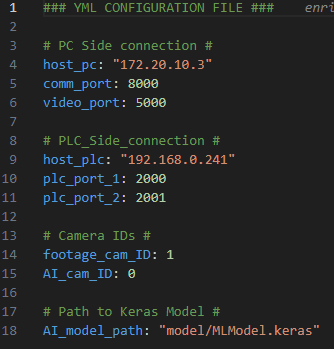
\includegraphics[scale=0.7]{images/yml.png}
        \centering
        \caption{The configuration file}
        \end{figure}
        The configuration file is a YML file that contains the parameters related to:
        \begin{itemize}
            \item IP address and ports of the interface through which the server connects to the client;
            \item IP address and ports of the interface through which the server connects to the PLC;
            \item The IDs with which openCV identifies the webcams used by the system (usually ID 0 is reserved for the computer built-in one, so it is necessary to pay particular attention when setting these parameters);
            \item The path of the Keras model that makes the predictions.
        \end{itemize}
        The parameters are automatically taken via the Python yml library, making the system modular (for example, the AI model can be easily replaced with another to perform a different task, simply by creating a new model and passing its path) and easy to configure.
        \subsection{Ladder diagram}
        To create the system and ensure its correct functioning, modifications were made to the original ladder diagram~\cite{ladder}. In particular:
        \begin{itemize}
            \item a new line was inserted to control the conveyor belt (Figure~\ref{conv_handle}), dependent on the output of the proximity sensor. If the proximity sensor detects an object, the conveyor belt is stopped. Once the object has been picked up, the conveyor starts moving again after 3 seconds thanks to the presence of a TOFF timer. Since the output of the sensor is, normally (when there is no object in its detection range), 24 V, a NC relay input was used. When the object is removed from the sensor detection field, the conveyor continues to remain stationary because the TOFF timer keeps the output line high for another 3 seconds;
            \item a socket (client) block was inserted (Figure~\ref{sensor_socket}) to allow the PLC to notify the presence of an object to the server machine. The socket connects to the server when the physical start button is pressed;
            \item a TSEND block (Figure~\ref{tsend}) was inserted, which sends a "start" string to the server as soon as the StopConveyor output becomes high, i.e. when an object is detected by the proximity sensor. This implements the server notification mechanism;
            \item a TDISCON block (Figure~\ref{tdiscon}) has been inserted to manage the disconnection of the PLC from the server, which is carried out when the physical Stop button is pressed.
        \end{itemize}

        \begin{figure}[H]
        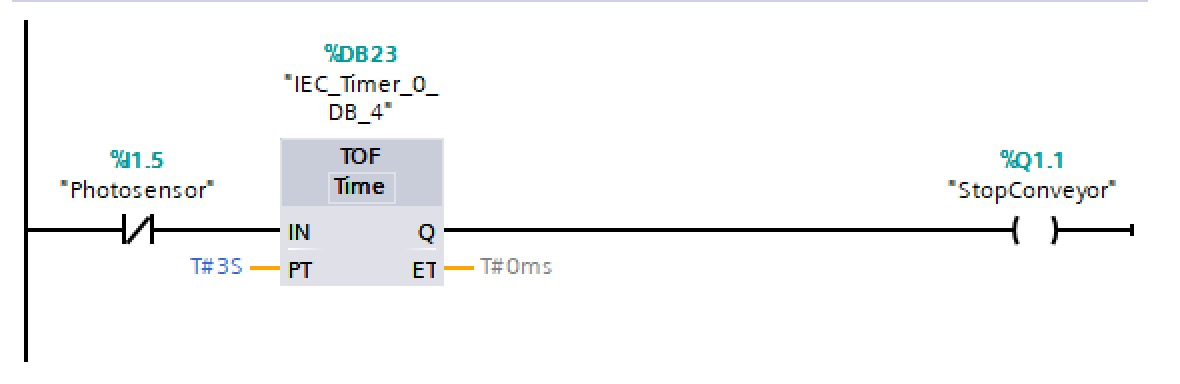
\includegraphics[scale=0.3]{images/CONV_HANDLE.jpeg}
        \centering
        \caption{Conveyor belt control line}
        \label{conv_handle}
        \end{figure}

        \begin{figure}[H]
        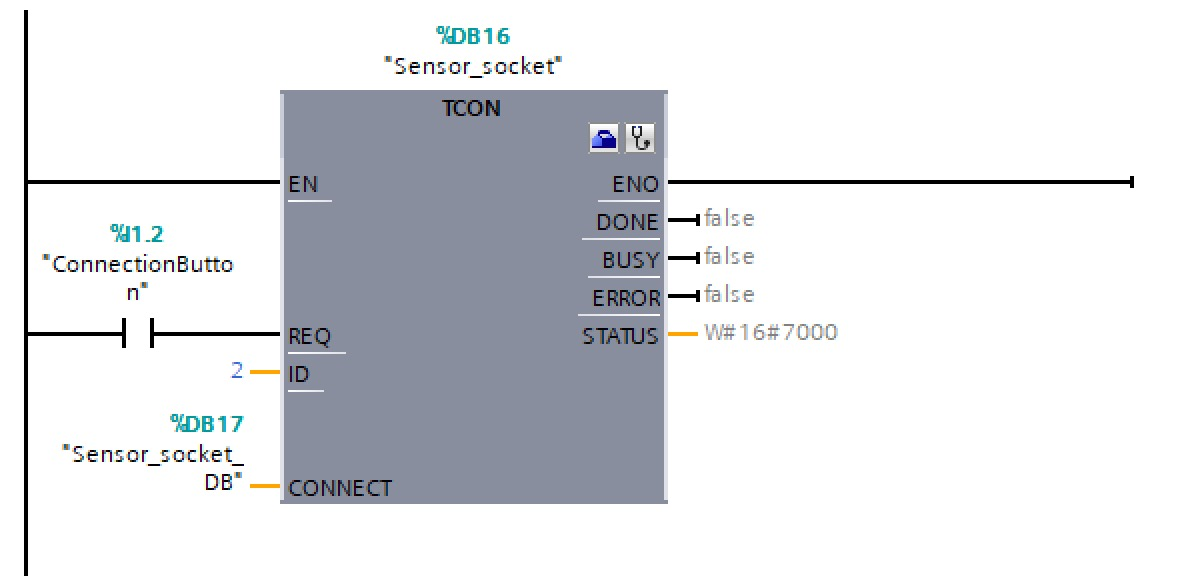
\includegraphics[scale=0.3]{images/SENSOR_SOCKET.jpeg}
        \centering
        \caption{Socket block}
        \label{sensor_socket}
        \end{figure}

        \begin{figure}[H]
        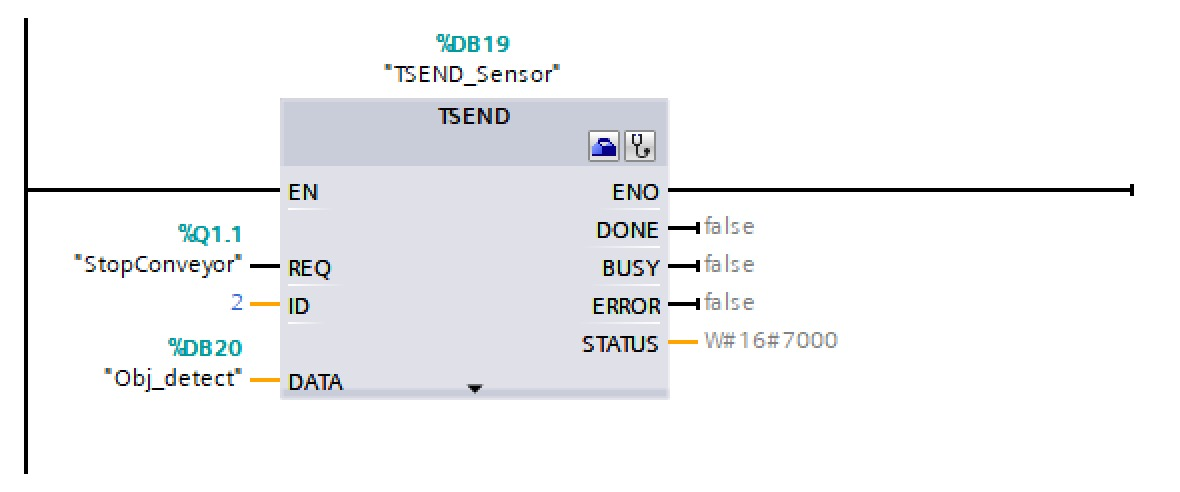
\includegraphics[scale=0.3]{images/TSEND.jpeg}
        \centering
        \caption{TSEND block}
        \label{tsend}
        \end{figure}

        \begin{figure}[H]
        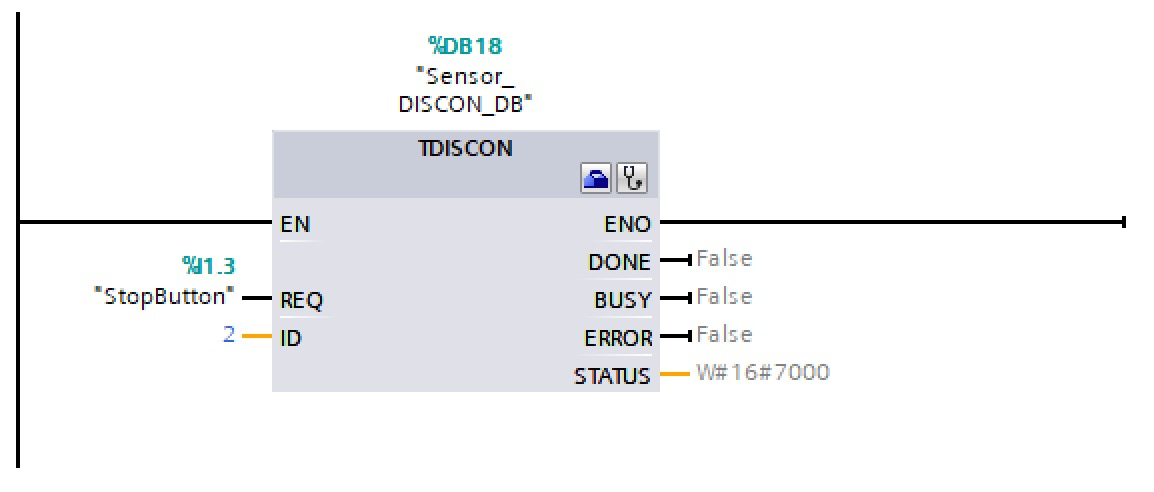
\includegraphics[scale=0.3]{images/TDISCON.jpeg}
        \centering
        \caption{TDISCON block}
        \label{tdiscon}
        \end{figure}
        


\begin{thebibliography}{99}
\bibitem{github}
    Project Github Repository \url{https://github.com/enrikata/IAAR-Project/tree/main}
\bibitem{githubvecchio}
   Previous robot project \url{https://github.com/giorgionocera/fischertechnik-3D-robot/tree/main}
\bibitem{schematic}
    Final schematic of the previous robot project
    \url{https://github.com/giorgionocera/fischertechnik-3D-robot/blob/main/documentation/capitolo3/figure/final_schematic.png}
\bibitem{ladder}
    Ladder diagram of the previous robot project
    \url{https://github.com/giorgionocera/fischertechnik-3D-robot/tree/main/tia%20portal/Project_v3_nuovo}
\bibitem{sheetsensor}
    Photoelectric sensor datasheet (E3F2-DS10C4) \url{https://datasheetspdf.com/pdf-file/555259/OmronElectronics/E3F2-DS10C4/1}
\bibitem{githubdata}
    Dataset generator Github repository \url{https://github.com/elkorchi/2DGeometricShapesGenerator}
\bibitem{matlab}
    Matlab code converted in python code \url{https://github.com/giorgionocera/fischertechnik-3D-robot/blob/main/matlab/move_robot.m}
\end{thebibliography}


\end{document}
